\documentclass{article}

\PassOptionsToPackage{numbers,sort&compress}{natbib}
\usepackage[preprint]{neurips2026/neurips_2026}
\usepackage[utf8]{inputenc}
\usepackage[T1]{fontenc}
\usepackage{hyperref}
\usepackage{url}
\usepackage{booktabs}
\usepackage{amsmath,amsfonts,amssymb}
\usepackage{nicefrac}
\usepackage{microtype}
\usepackage{xcolor}
\usepackage{graphicx}
\usepackage{enumitem}
\usepackage{multirow}
\usepackage{array}
\usepackage{wrapfig}

\newcommand{\miou}{\ensuremath{\mathrm{mIoU}}}
\newcommand{\iou}{\ensuremath{\mathrm{IoU}}}
\newcommand{\ignore}{\ensuremath{y=255}}
\newcommand{\code}[1]{\texttt{#1}}
\setlist{nosep,leftmargin=1.4em}

\title{AresSeg: A Controlled Study of CNNs, Transformers, and Foundation Models for Mars Terrain Segmentation}

\author{%
  John Roth\\
  EN.705.742 Advanced Applied Machine Learning\\
  Summer 2026\\
  \texttt{jroth1414/AresSeg}
}

\begin{document}
\maketitle

\begin{abstract}
Reliable terrain perception can increase the safety and autonomy of Mars rover traverses, but
architecture comparisons are easily confounded by data splits, initialization, and incomplete
uncertainty estimates. We present AresSeg, a controlled four-class semantic-segmentation study on
AI4Mars Navcam imagery. Thirty learned runs compare U-Net, DeepLabV3+, SegFormer, a small U-Net,
and a satellite-pretrained DINOv3 model at three seeds; a parameter-free majority predictor and
the Segment Anything Model (SAM) region-oracle serve as references. All systems share a
leakage-safe split, ignore-label handling, objective, expert test sets, and a preregistered paired
seed/image bootstrap with Holm correction. Conventional systems reach mean Curiosity test
\miou{} of 0.810--0.824 and all exceed the training-derived majority baseline by at least 0.754
(adjusted $p<0.001$). We find no corrected evidence that ImageNet initialization improves a tested
architecture and no corrected overall or class-specific difference between the configured
SegFormer-B2 and CNN systems. The validation-selected U-Net transfers from Curiosity to
Opportunity/Spirit with mean \miou{} 0.792, a 0.030 drop and 90\% interval $[0.725,0.848]$, thereby
satisfying the prespecified robustness rule. DINOv3-SAT obtains the highest mean \miou{} (0.836)
and significantly exceeds Tiny U-Net by 0.148, whereas SAM's label-assisted region upper bound
does not. These results favor careful representation transfer and compact SegFormer-B0 efficiency
over a simple CNN-versus-transformer narrative.
\end{abstract}

\section{Introduction}

Mars rovers operate under communication latency, intermittent contact, and strict safety margins.
Longer autonomous drives require immediate understanding of the surface ahead: sand may induce
slip, embedded bedrock contributes to wheel wear, and large rocks are direct hazards. SPOC linked
deep terrain classification to operational rover mobility \cite{rothrock2016spoc}, while AI4Mars
made large-scale pixel supervision available by combining crowdsourced labels with expert test
annotations \cite{swan2021ai4mars}. The remaining practical question is not merely whether a
network can segment Mars terrain, but which representation transfers reliably under controlled
evaluation and rover shift.

This paper asks: \emph{How do convolutional, transformer, and foundation-model systems compare on
four-class Mars terrain segmentation; does pretrained initialization help; and does a
Curiosity-selected system generalize to Opportunity/Spirit imagery?} We study soil, bedrock, sand,
and big rock in grayscale Curiosity Navcam images, with label 255 excluded from both loss and
metrics. The study contributes:

\begin{enumerate}
  \item a camera-scoped, leakage-safe AI4Mars pipeline with reconstructable per-image statistics;
  \item a matched three-seed comparison of CNNs, hierarchical transformers, initialization, and
  two foundation-model references;
  \item a held-out Curiosity-to-MER transfer test with preregistered selection and decision rules;
  \item a fully sealed analysis trail that records protocol amendments rather than rewriting them.
\end{enumerate}

The visual summary in Figure~\ref{fig:qual-msl} previews the central empirical pattern: several
learned systems produce strong broad-terrain maps, yet rare rocks and class boundaries remain
visually and statistically harder than soil or bedrock.

\begin{figure}[t]
  \centering
  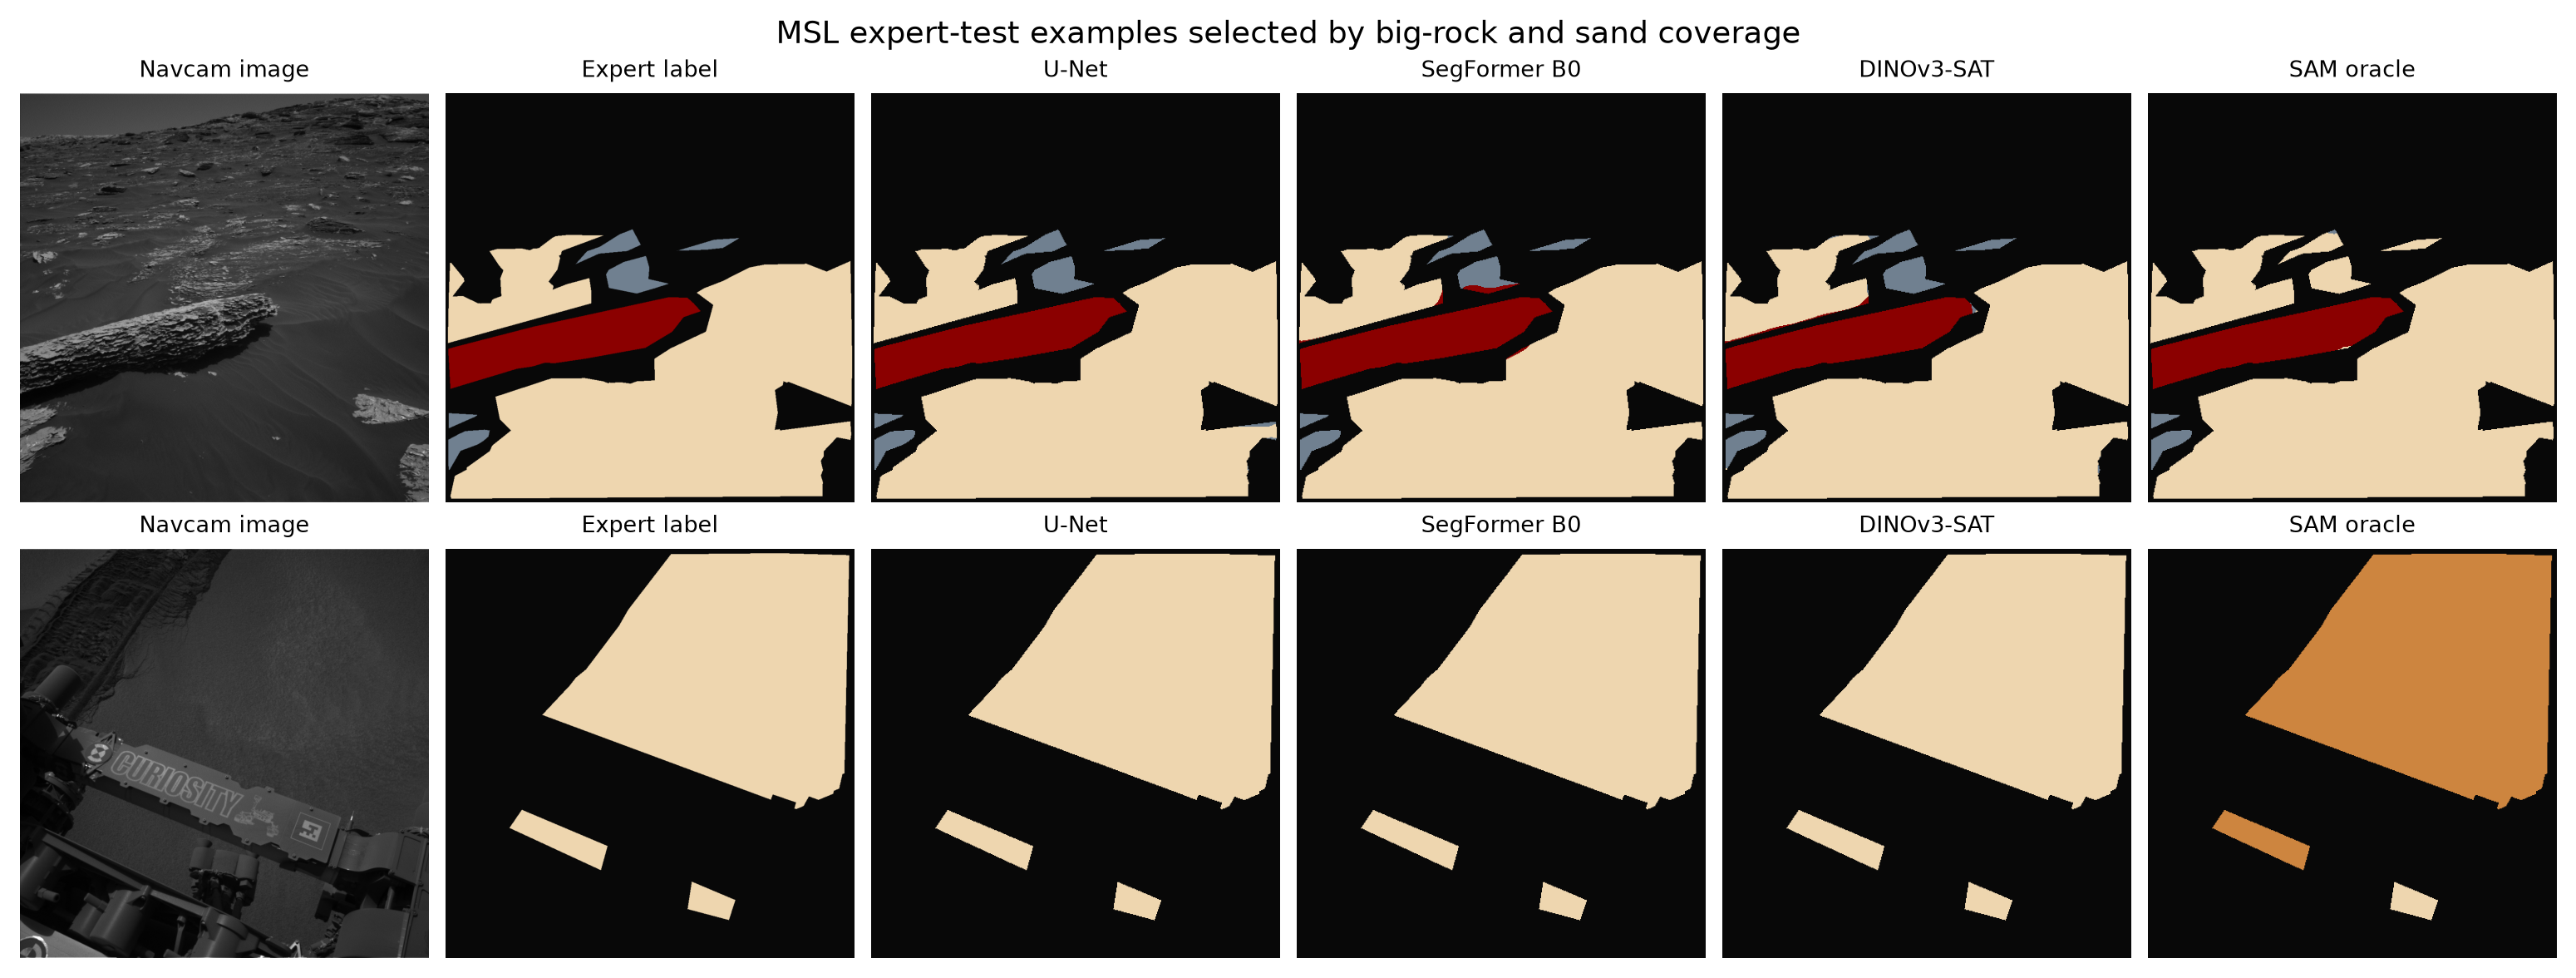
\includegraphics[width=\textwidth]{figures/final/qualitative_msl.png}
  \caption{Two Curiosity expert-test scenes selected deterministically for high big-rock (top) and
  sand (bottom) coverage. SAM is a label-assisted region-oracle upper bound, not a deployable
  semantic classifier. All colors use one fixed terrain palette; black denotes ignored pixels.}
  \label{fig:qual-msl}
\end{figure}

\section{Related work}

\paragraph{Mars terrain perception.}
AI4Mars contains rover imagery, crowdsourced training labels, and expert evaluation labels from
Curiosity, Spirit, and Opportunity \cite{swan2021ai4mars}; this work uses its merged-0.6 public
release \cite{ai4marszenodo}. SPOC previously demonstrated operationally motivated terrain
classification for Mars rover missions \cite{rothrock2016spoc}. MarsSeg explores Mars-specific
multi-level feature extraction, but remains a research preprint \cite{li2024marsseg}. Our focus is
complementary: controlled comparisons, initialization effects, cross-rover transfer, and paired
inference under one protocol.

\paragraph{CNN and transformer segmentation.}
Fully convolutional prediction established end-to-end dense recognition \cite{long2015fcn}.
U-Net recovers spatial detail through encoder--decoder skip connections
\cite{ronneberger2015unet}, whereas DeepLabV3+ combines atrous multi-scale context with a boundary
refinement decoder \cite{chen2018deeplab}. Residual/ImageNet encoders offer reusable visual priors
\cite{he2016resnet,deng2009imagenet}. Vision Transformers replace local convolution with
patch-token attention \cite{dosovitskiy2021vit}; SegFormer adapts this idea to efficient
hierarchical dense prediction \cite{xie2021segformer}. Because each family changes capacity and
optimization as well as inductive bias, our H3 conclusions concern configured systems, not a pure
causal effect of attention.

\paragraph{Foundation references.}
SAM learns class-agnostic object masks at scale \cite{kirillov2023sam}, but AI4Mars supplies no
prompt-to-terrain semantic channel. We therefore use the frozen region-oracle rule only as an
upper bound on its proposal partition. DINOv3 is a 2025 technical report, not a peer-reviewed
paper \cite{simeoni2025dinov3}. Its SAT-493M representation is nevertheless a useful stress test:
it transfers self-supervised features from Earth orbital imagery to ground-level Mars imagery.

\section{Problem and hypotheses}

For an image $x\in\mathbb{R}^{H\times W}$, replicated to three channels for pretrained encoders,
a model $f_\theta$ produces four logits per pixel. The prediction is
\begin{equation}
  \hat y_{ij}=\arg\max_{c\in\{0,1,2,3\}} f_\theta(x)_{ijc}.
\end{equation}
Pixels satisfying \ignore{} are invalid and contribute to neither optimization nor sufficient
statistics. Class IoU and the primary macro mean are
\begin{equation}
  \mathrm{IoU}_c=\frac{\mathrm{TP}_c}{\mathrm{TP}_c+\mathrm{FP}_c+\mathrm{FN}_c},
  \qquad \miou=\frac{1}{|S|}\sum_{c\in S}\mathrm{IoU}_c,
\end{equation}
where $S$ is the fixed set of classes present in the full evaluation split.

The sealed hypotheses are: H0, no tested deep system beats constant majority; H1, at least one
conventional deep system does; H2, pretraining improves at least one backbone-matched system; H3,
configured SegFormer-B2 and CNN systems differ overall or by class; H4, the validation-selected
system has cross-rover drop $<0.15$ and an MER confidence lower bound above MER majority; and H5,
DINOv3-SAT or the SAM upper bound exceeds Tiny U-Net. H0 is rejected exactly when H1 is supported.
Failure of H2 or H3 is not interpreted as proof of equivalence.

\section{Method}

\subsection{Data and leakage controls}

The MSL Navcam index contains 16,064 labeled training images and 322 expert-test images. A
seed-1414 by-image split yields 12,851 training and 3,213 validation records; no crop or frame
crosses partitions. The independent MER expert set contains 204 Opportunity/Spirit images and is
never used for fitting or selection. Preflight verifies counts, image--label pairing, split
disjointness, the vocabulary $\{0,1,2,3,255\}$, source checksum, and a path/size index fingerprint.
The dataset is not copied into the repository; the public record and expected MD5 are documented.

Images are resized to $512^2$, replicated to RGB, and ImageNet-normalized. Training uses
horizontal flip and mild brightness/contrast perturbation; physically implausible vertical flips
are disabled. Masks use nearest-neighbor resizing. Median-frequency class weights are clipped to
$[0.5,10]$ and computed only from the training split.

\subsection{Systems and optimization}

The 30 learned runs comprise Tiny U-Net; U-Net--ResNet34; DeepLabV3+--ResNet50; SegFormer MiT-B0
and B2, each where applicable with ImageNet and random initialization; and DINOv3-SAT ViT-L/16
with a trained segmentation head. The deterministic training-pixel majority predictor selects
bedrock (class 1); its full count evidence is sealed in Protocol V5. SAM ViT-B assigns each
generated proposal its majority valid target class and defaults uncovered pixels to soil, making
it explicitly label-assisted.

Learned systems minimize weighted cross-entropy plus soft Dice loss
\cite{milletari2016vnet}:
\begin{equation}
  \mathcal{L}=\mathcal{L}^{w}_{\mathrm{CE}}+
  \left(1-\frac{2\sum p g+\epsilon}{\sum p+\sum g+\epsilon}\right),
\end{equation}
with the validity mask applied to both terms. AdamW uses learning rate $3\times10^{-4}$, weight
decay $10^{-4}$, batch size 8, at most 50 epochs, gradient clipping at 1.0, and early stopping
patience 10 \cite{loshchilov2019adamw}. The best validation-\miou{} checkpoint is evaluated once.

\subsection{Statistical protocol and reproducibility}

Learned arms use seeds 1414, 1415, and 1416. For each comparison, 10,000 bootstrap replicates
resample training seeds and then paired images within seeds. We report percentile 90\% intervals
and plus-one $p$-values \cite{efron1993bootstrap}. Family A/B tests are one-sided; Family C is
two-sided and corrects both overall and four per-class tests across both comparisons. Holm
correction controls each preregistered family at $\alpha=0.10$ \cite{holm1979simple}; H4 uses its
threshold-plus-interval rule without a $p$-value.

Each run stores its resolved config, Git revision, code/config hashes, environment, parameter
counts, best validation score, and per-image intersections/unions. Protocol V5 SHA-256 is
\code{8485810bebed7d1396a0e8c065873ca56c6ea65565f3a919898d46509734ae04}. Thirty learned runs used
approximately 179.1 V100 device-hours (32 GB V100-SXM2), reconstructed from run start IDs and
manifest completion timestamps; the median run was 5.37 hours. Checkpoints and raw data remain
untracked.

\section{Results}

\subsection{Overall performance and capacity}

Figure~\ref{fig:overall} and Table~\ref{tab:models} summarize the complete inventory. DINOv3-SAT
has the highest mean test \miou{} (0.836), followed by scratch U-Net (0.824) and pretrained U-Net
(0.821). The ranking is descriptive; corrected comparisons below determine the claims. SegFormer
B0 is notable for reaching 0.814 with 3.7M parameters, roughly one-seventh of U-Net or
DeepLabV3+ and one-eightieth of DINOv3-SAT.

\begin{figure}[t]
  \centering
  \begin{minipage}[t]{0.58\textwidth}
    \centering
    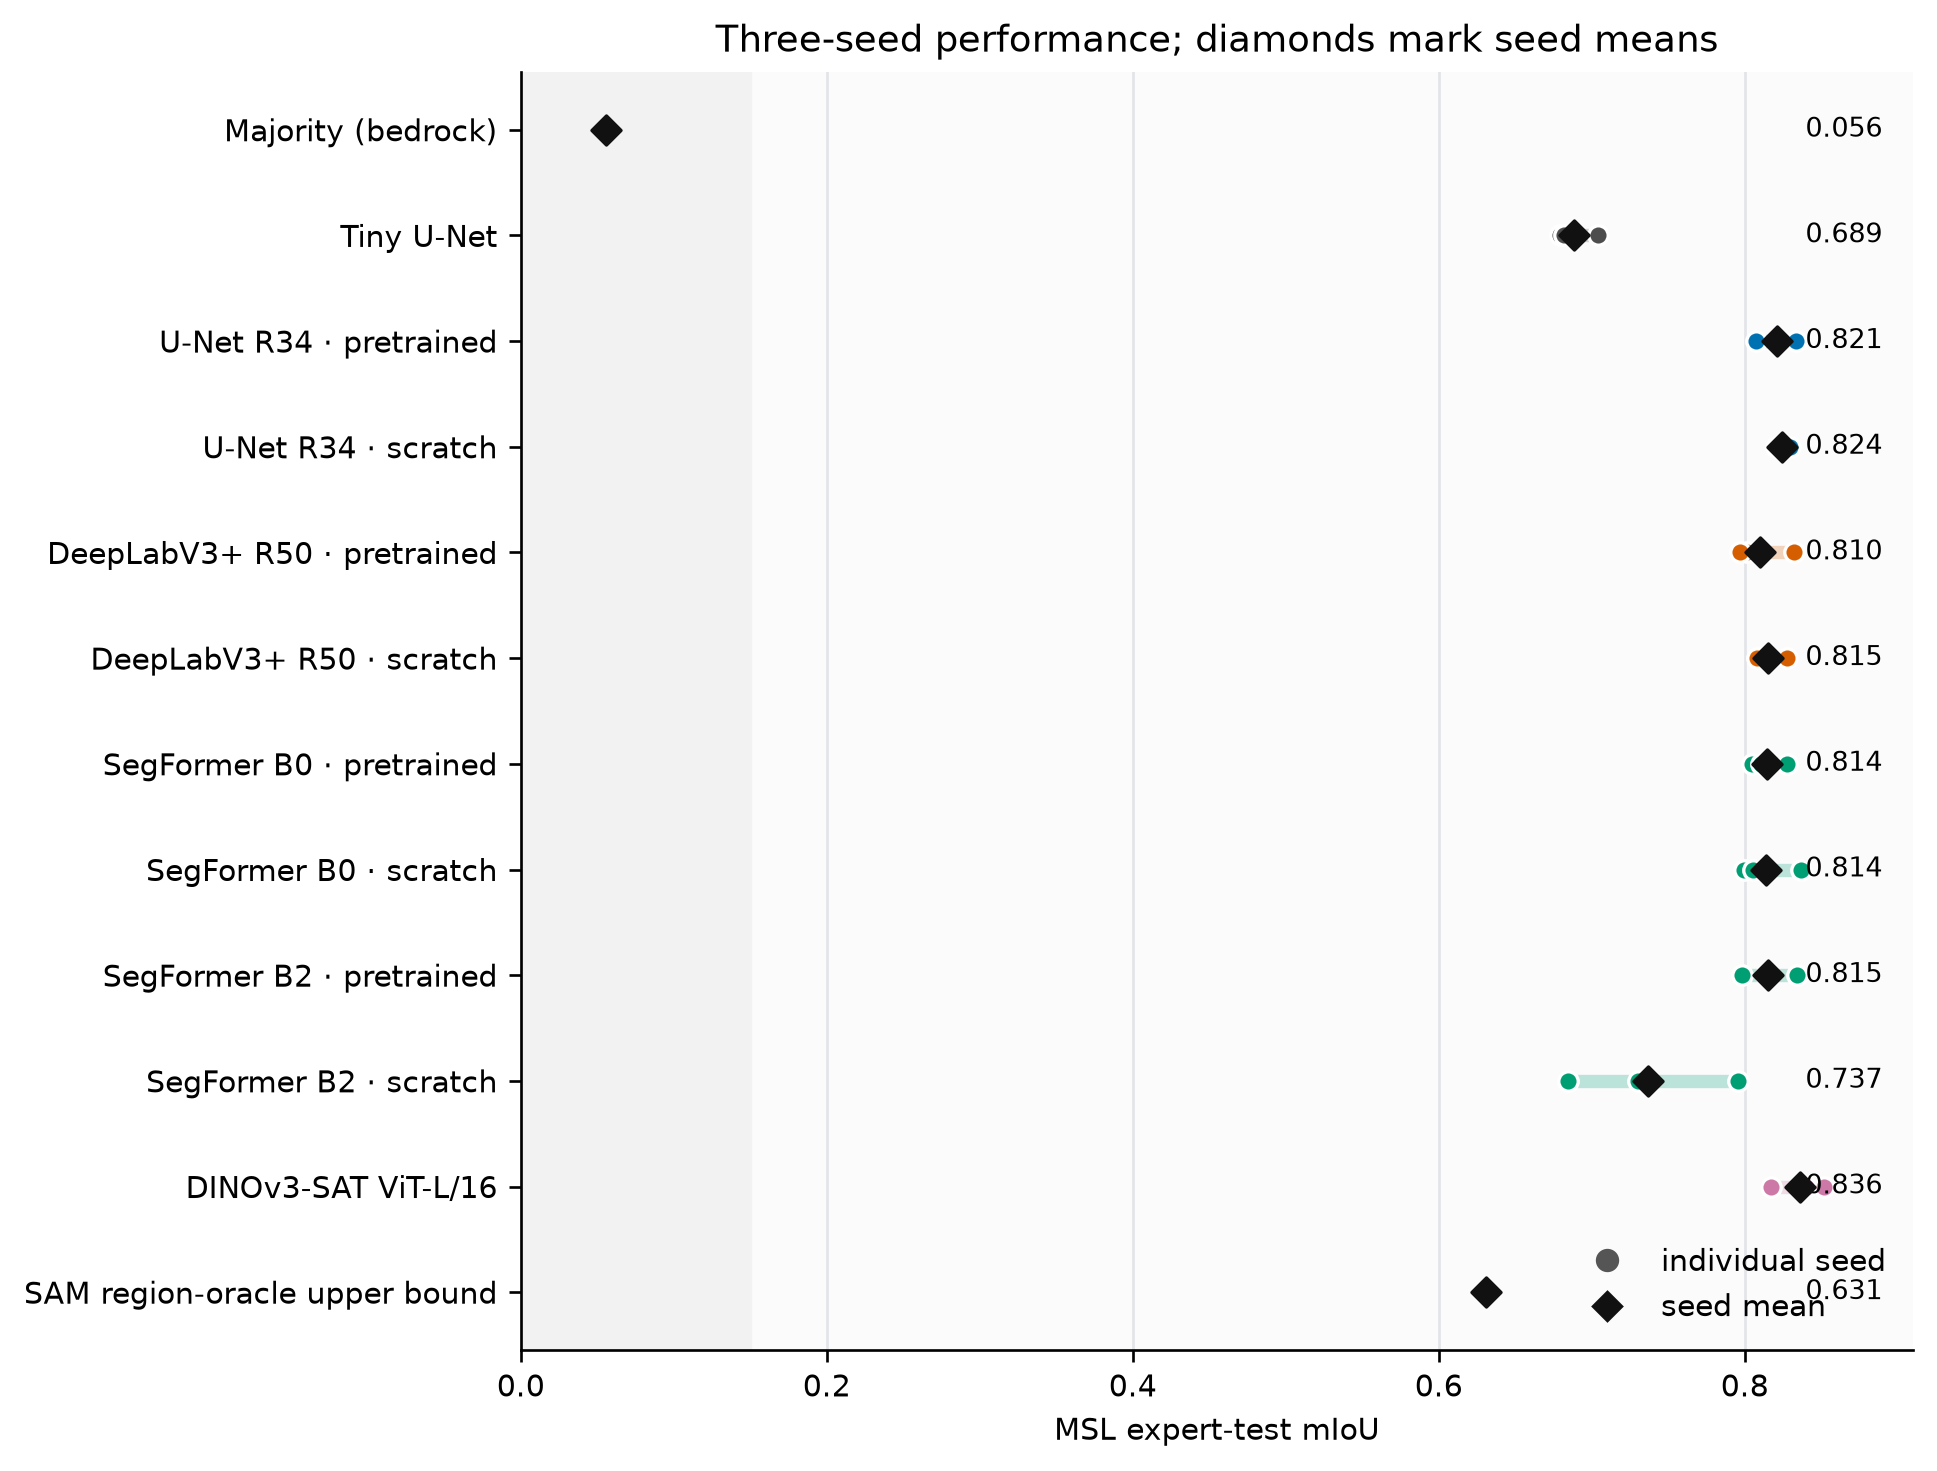
\includegraphics[width=\linewidth]{figures/final/performance_overview.png}
  \end{minipage}\hfill
  \begin{minipage}[t]{0.40\textwidth}
    \centering
    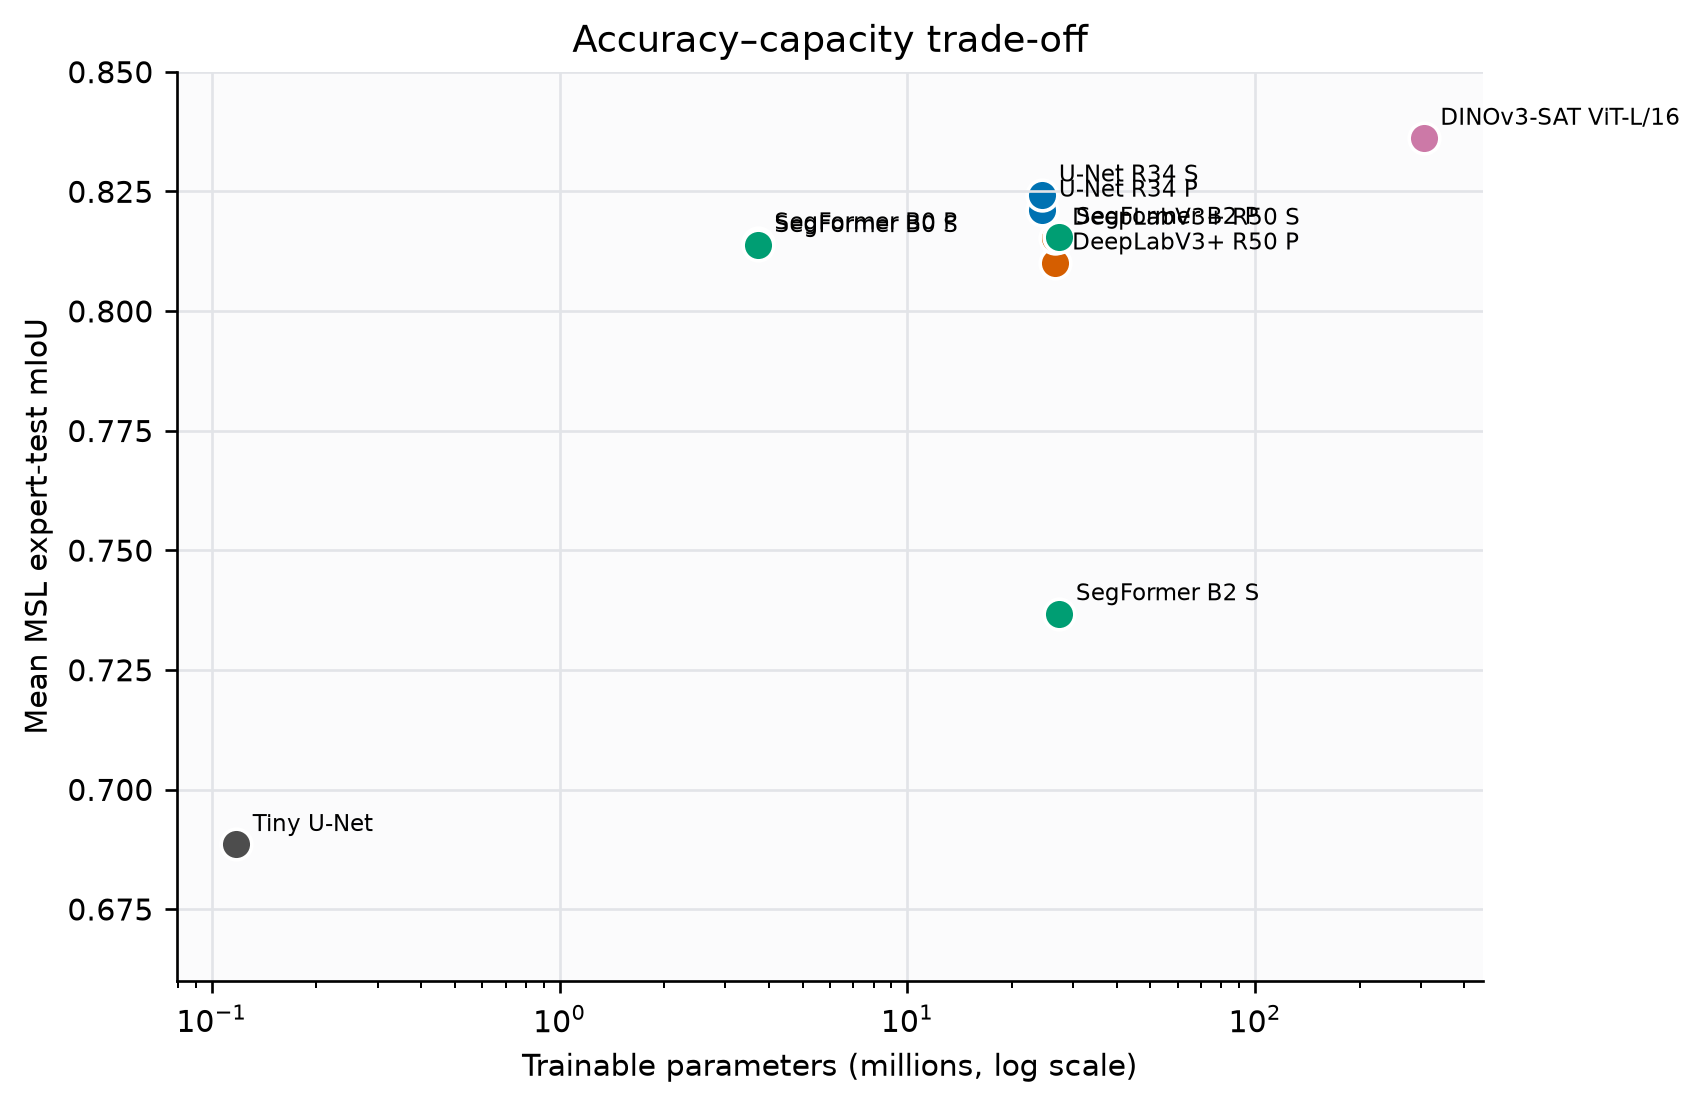
\includegraphics[width=\linewidth]{figures/final/parameter_efficiency.png}
  \end{minipage}
  \caption{Left: all completed MSL runs; diamonds are seed means and bars span seeds. Right:
  parameter efficiency for learned systems. SAM and majority are omitted from the capacity panel
  because their roles are not ordinary trained segmentation models.}
  \label{fig:overall}
\end{figure}

\begin{table}[t]
  \centering
  \caption{Expert-test performance. SD is across three training seeds; deterministic references
  are evaluated once. SAM is a label-assisted region upper bound.}
  \label{tab:models}
  \resizebox{\textwidth}{!}{\begin{tabular}{lrrr}
\toprule
System & Seeds & mIoU (mean $\pm$ SD) & Params \\
\midrule
Majority (bedrock) & 1 & 0.056 $\pm$ -- & 0 \\
Tiny U-Net & 3 & 0.689 $\pm$ 0.014 & 0.1M \\
U-Net R34 \textperiodcentered{} pretrained & 3 & 0.821 $\pm$ 0.013 & 24.4M \\
U-Net R34 \textperiodcentered{} scratch & 3 & 0.824 $\pm$ 0.005 & 24.4M \\
DeepLabV3+ R50 \textperiodcentered{} pretrained & 3 & 0.810 $\pm$ 0.019 & 26.7M \\
DeepLabV3+ R50 \textperiodcentered{} scratch & 3 & 0.815 $\pm$ 0.011 & 26.7M \\
SegFormer B0 \textperiodcentered{} pretrained & 3 & 0.814 $\pm$ 0.012 & 3.7M \\
SegFormer B0 \textperiodcentered{} scratch & 3 & 0.814 $\pm$ 0.020 & 3.7M \\
SegFormer B2 \textperiodcentered{} pretrained & 3 & 0.815 $\pm$ 0.018 & 27.3M \\
SegFormer B2 \textperiodcentered{} scratch & 3 & 0.737 $\pm$ 0.056 & 27.3M \\
DINOv3-SAT ViT-L/16 & 3 & 0.836 $\pm$ 0.018 & 305.5M \\
SAM region-oracle upper bound & 1 & 0.631 $\pm$ -- & 93.7M \\
\bottomrule
\end{tabular}
}
\end{table}

\subsection{Preregistered hypothesis tests}

All conventional systems strongly exceed majority: paired differences are 0.765 for U-Net, 0.754
for DeepLabV3+, and 0.758 for the validation-selected SegFormer-B0, with adjusted
$p=3.0\times10^{-4}$ for each. H1 is supported and H0 rejected. In contrast, pretraining effects
are $-0.003$ (U-Net), $-0.005$ (DeepLabV3+), and $+0.001$ (SegFormer-B0); every 90\% interval
crosses zero and all adjusted $p\geq0.594$. H2 is rejected without claiming equivalence.

SegFormer-B2 differs from U-Net by $-0.006$ \miou{} and from DeepLabV3+ by $+0.005$; neither is
significant. None of the eight class-specific Family-C tests survives correction (all adjusted
$p=1$), so H3 is rejected. Figure~\ref{fig:inference} displays all overall effects and asymmetric
bootstrap intervals. Table~\ref{tab:hypotheses} gives the final hypothesis-level decisions.

\begin{figure}[t]
  \centering
  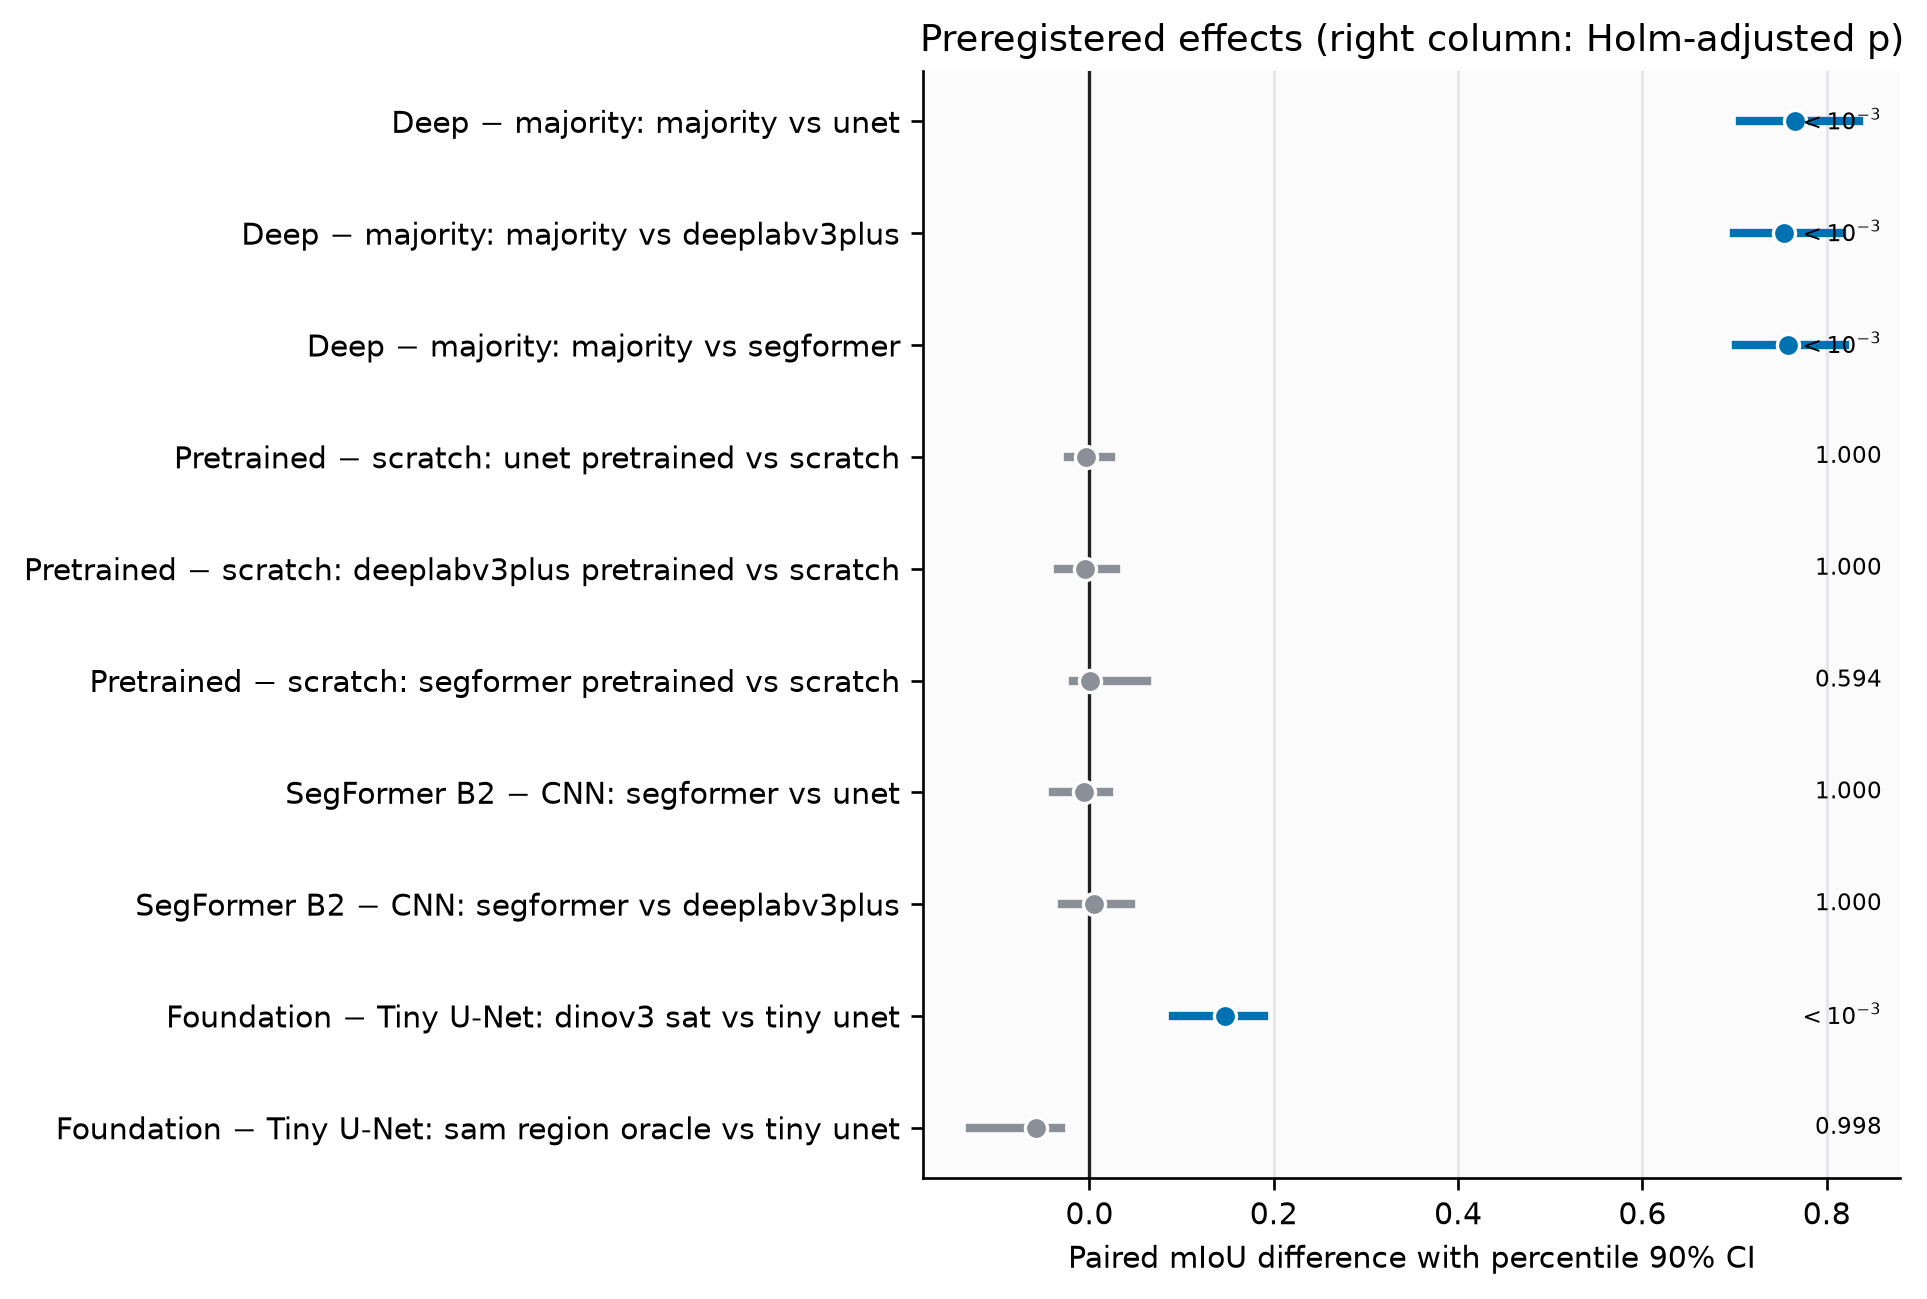
\includegraphics[width=0.93\textwidth]{figures/final/hypothesis_forest.png}
  \caption{Paired effect estimates. Positive values favor the first named side of each
  comparison. Blue marks corrected significance; gray marks nonsignificance. Family C per-class
  tests are reported in the appendix.}
  \label{fig:inference}
\end{figure}

\begin{table}[t]
  \centering
  \caption{Final preregistered decisions. ``Rejected'' means the prespecified support rule was not
  met, not evidence of model equivalence.}
  \label{tab:hypotheses}
  \resizebox{0.92\textwidth}{!}{\begin{tabular}{llll}
\toprule
Hypothesis & Decision & Key evidence & Adjusted $p$ \\
\midrule
H0 & Rejected & H1 supported & -- \\ 
H1 & Supported & $\Delta$=0.754--0.765 & $<0.001$ \\ 
H2 & Rejected & all transfer CIs cross 0 & $\geq0.594$ \\ 
H3 & Rejected & all 10 tests nonsignificant & 1.000 \\ 
H4 & Supported & drop=0.030; MER CI$_L$=0.725 & rule \\ 
H5 & Supported & DINOv3 $\Delta$=0.148 & $<0.001$ \\ 
\bottomrule
\end{tabular}
}
\end{table}

\subsection{Terrain classes, rover shift, and foundation models}

The heatmap in Figure~\ref{fig:class-h4} shows that strong aggregate scores coexist with weaker and
more variable big-rock recognition. The validation-selected pretrained U-Net has mean MSL
\miou{} 0.821 and mean MER \miou{} 0.792. Its drop is only 0.030; the hierarchical MER 90\%
interval is $[0.725,0.848]$, whose lower bound is far above MER majority (0.068). H4 is supported,
although seed 1416's MER score (0.714) cautions against a single-run transfer claim.

DINOv3-SAT exceeds Tiny U-Net by 0.148 with interval $[0.091,0.190]$ and adjusted
$p=2.0\times10^{-4}$. SAM's region-oracle scores only 0.631 and is 0.058 below Tiny U-Net; its
one-sided comparison is not significant. H5 is supported through DINOv3, not through SAM. This
distinction matters: strong class-aware features transfer across planets, while generic object
partitioning alone does not solve terrain semantics.

\begin{figure}[t]
  \centering
  \begin{minipage}[t]{0.56\textwidth}
    \centering
    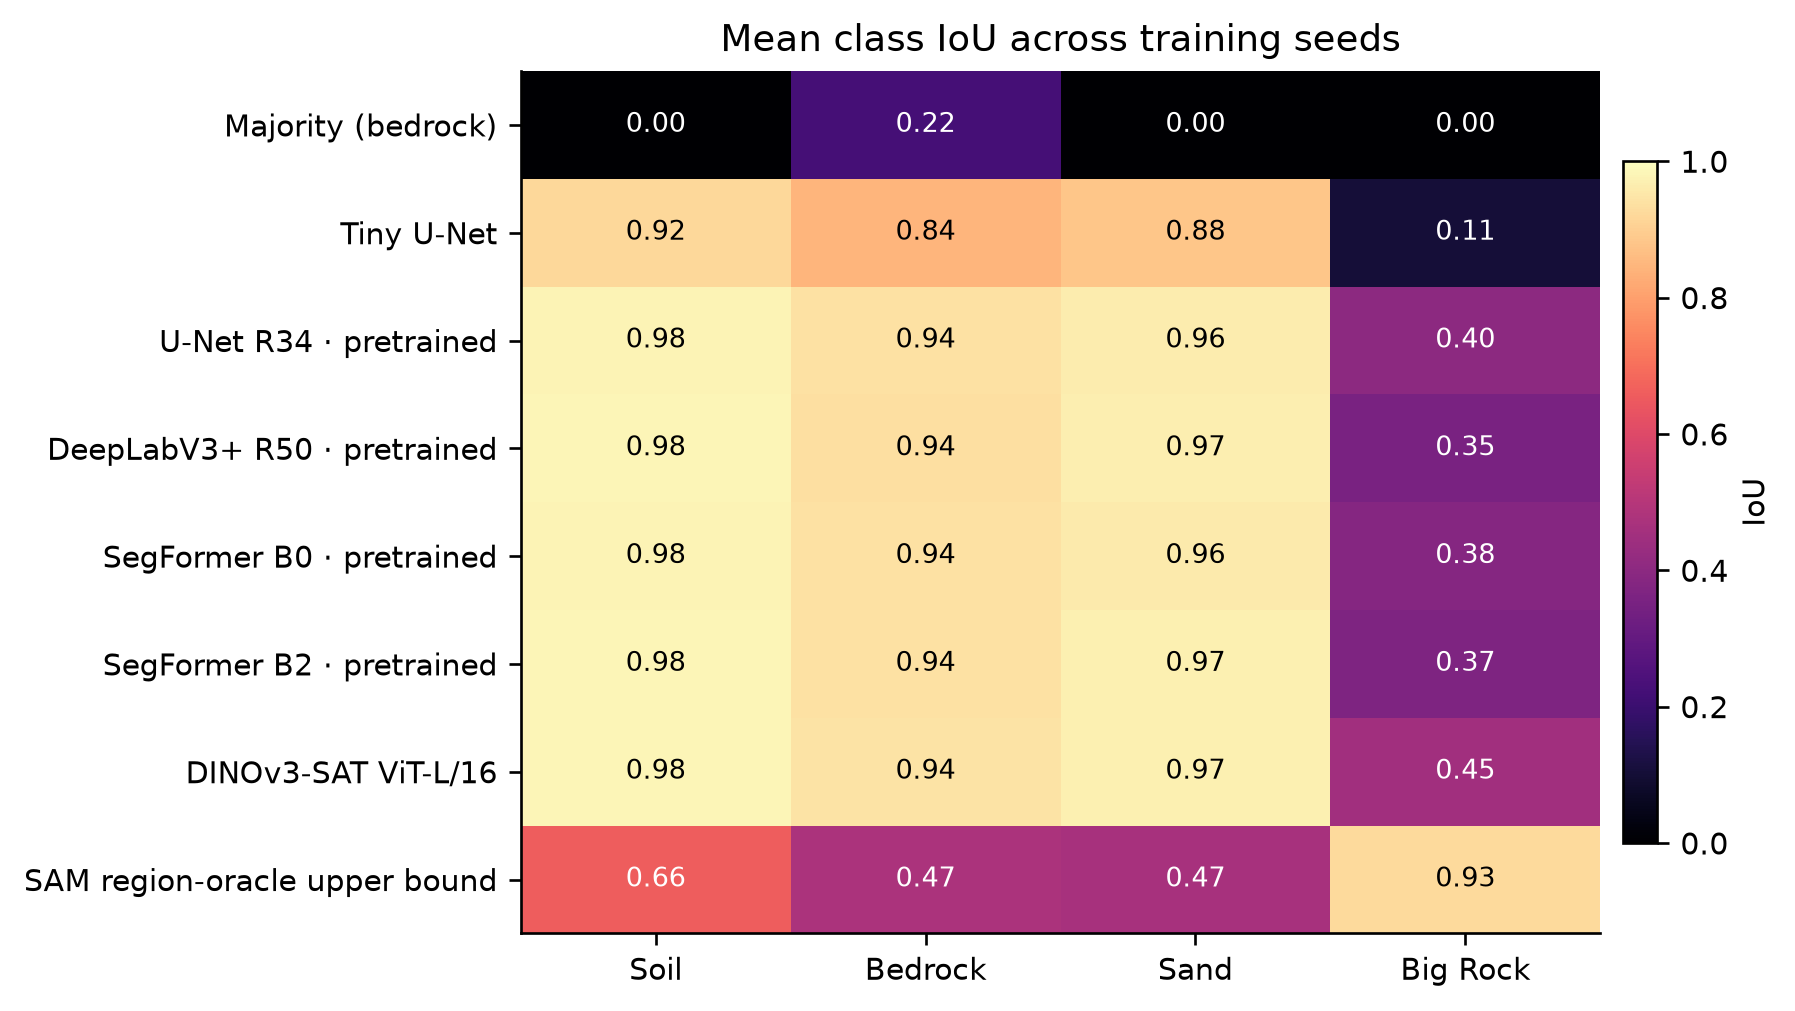
\includegraphics[width=\linewidth]{figures/final/per_class_heatmap.png}
  \end{minipage}\hfill
  \begin{minipage}[t]{0.42\textwidth}
    \centering
    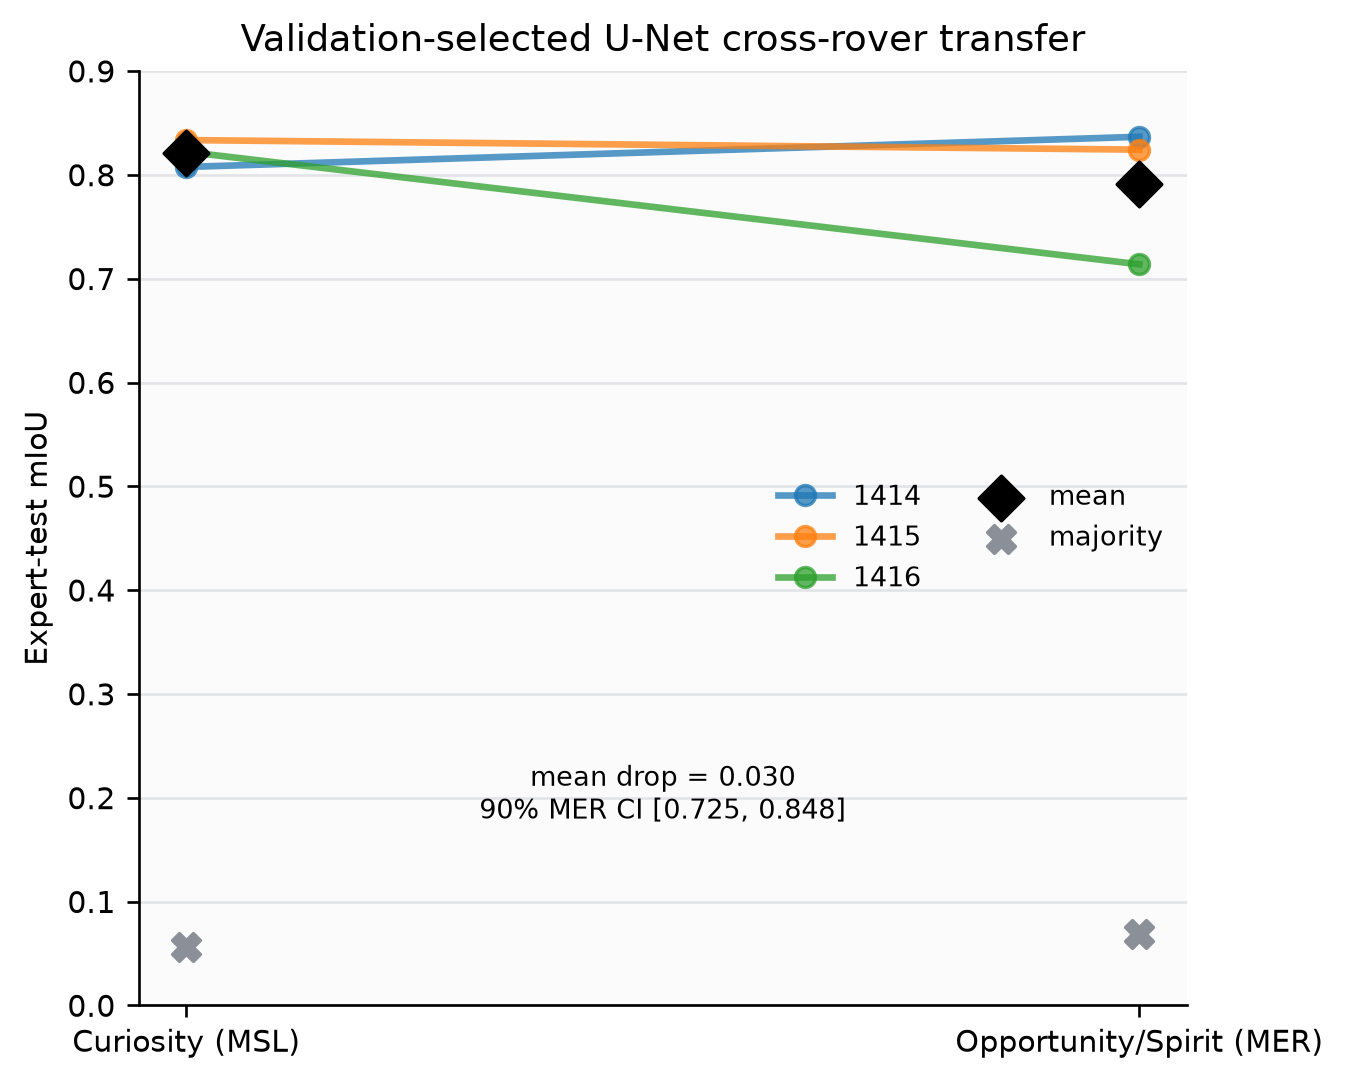
\includegraphics[width=\linewidth]{figures/final/cross_rover_generalization.png}
  \end{minipage}
  \caption{Left: mean terrain-class IoU. Right: paired Curiosity and MER U-Net results, with
  training-derived majority references. Diamonds denote means.}
  \label{fig:class-h4}
\end{figure}

\section{Discussion}

The evidence does not support a simple claim that transformers beat CNNs, or that ImageNet
initialization universally helps. U-Net, DeepLabV3+, and both SegFormer sizes occupy a narrow
performance band after three seeds; configured-system differences are small relative to
image-level and seed uncertainty. Scratch SegFormer-B2 is an exception with high variability,
suggesting that the larger transformer is harder to optimize from random initialization, but the
pretraining family as formally defined still does not pass correction.

DINOv3-SAT provides the clearest positive transfer result despite the largest viewpoint and
planetary domain gap. Its advantage over Tiny U-Net does not establish superiority to all
conventional systems, but it does show that large-scale self-supervised satellite features remain
useful after adaptation. Conversely, SAM's target-assisted region upper bound underperforms Tiny
U-Net; an autonomous class labeler could only do worse under this proposal partition. Semantic
terrain representation, not mask granularity alone, appears to be the decisive ingredient.

Cross-rover transfer is encouraging but uneven. Mean degradation meets a strict bound and MER
performance remains far above majority, yet the weakest seed falls more than 0.10 below the other
two. Operational use should therefore ensemble or calibrate across conditions rather than deploy a
single checkpoint on the basis of mean \miou{}. Rare big-rock uncertainty is also more safety
relevant than another small improvement on soil.

\section{Limitations and broader impacts}

The scope is one public dataset release, grayscale Navcam imagery, four coarse classes, and three
training seeds. MER shift entangles rover, camera, mission, illumination, and geography, so it does
not isolate a causal domain factor. Crowdsourced training labels contain ambiguity even though the
test subset requires expert agreement. Macro \miou{} weights rare classes equally at aggregation,
but rare big-rock pixels still yield wider uncertainty. SAM's oracle consults targets and is not
deployable. DINOv3-SAT is a large preprint model whose compute cost limits onboard use; SegFormer-B0
is the more plausible efficiency candidate. The exploratory MPBA screen was validation-only and
not promoted, so it cannot support a gold-test claim.

Safer perception could enable more productive planetary exploration, but segmentation errors may
also encourage unsafe autonomous plans. This work is not a flight-qualified navigation system:
deployment would require calibrated uncertainty, hardware timing, hazard-aware planning,
simulation, Earth-analog field trials, and mission verification. The study contains no personal
data and introduces no surveillance application. The merged dataset archive credits NASA/JPL and
Zooniverse, but does not state an explicit license in its bundled metadata; downstream reuse should
verify current record terms.

\section{Conclusion}

Under one leakage-safe, three-seed protocol, conventional CNN and transformer systems all perform
strongly and decisively beat majority, but neither ImageNet pretraining nor configured
CNN--transformer differences survive multiplicity correction. A validation-selected U-Net meets
the preregistered Curiosity-to-MER robustness rule. DINOv3-SAT yields the highest mean score and
supports H5, while SAM proposals alone do not. The most defensible next experiment is therefore a
compact DINO-style or SegFormer-B0 representation with explicit uncertainty and rare-rock
objectives, evaluated on new rover and lighting strata rather than another unconstrained
architecture ranking.

\section*{Data and code availability}

AI4Mars merged-0.6 is available through Zenodo record 15995036
\cite{ai4marszenodo}; the expected archive is approximately 16.2 GB with MD5
\code{daf80a86021253292e6c425f97baa5c6}. The public AresSeg repository includes acquisition and
integrity instructions, exact configs, protocol seals, compact result stores, manifests,
per-image sufficient statistics, analysis code, figures, and a CPU-runnable notebook. Raw data,
secrets, checkpoints, and generated prediction rasters are intentionally excluded.

\bibliographystyle{plainnat}
\bibliography{references}

\appendix

\section{Additional qualitative results}

\begin{figure}[h]
  \centering
  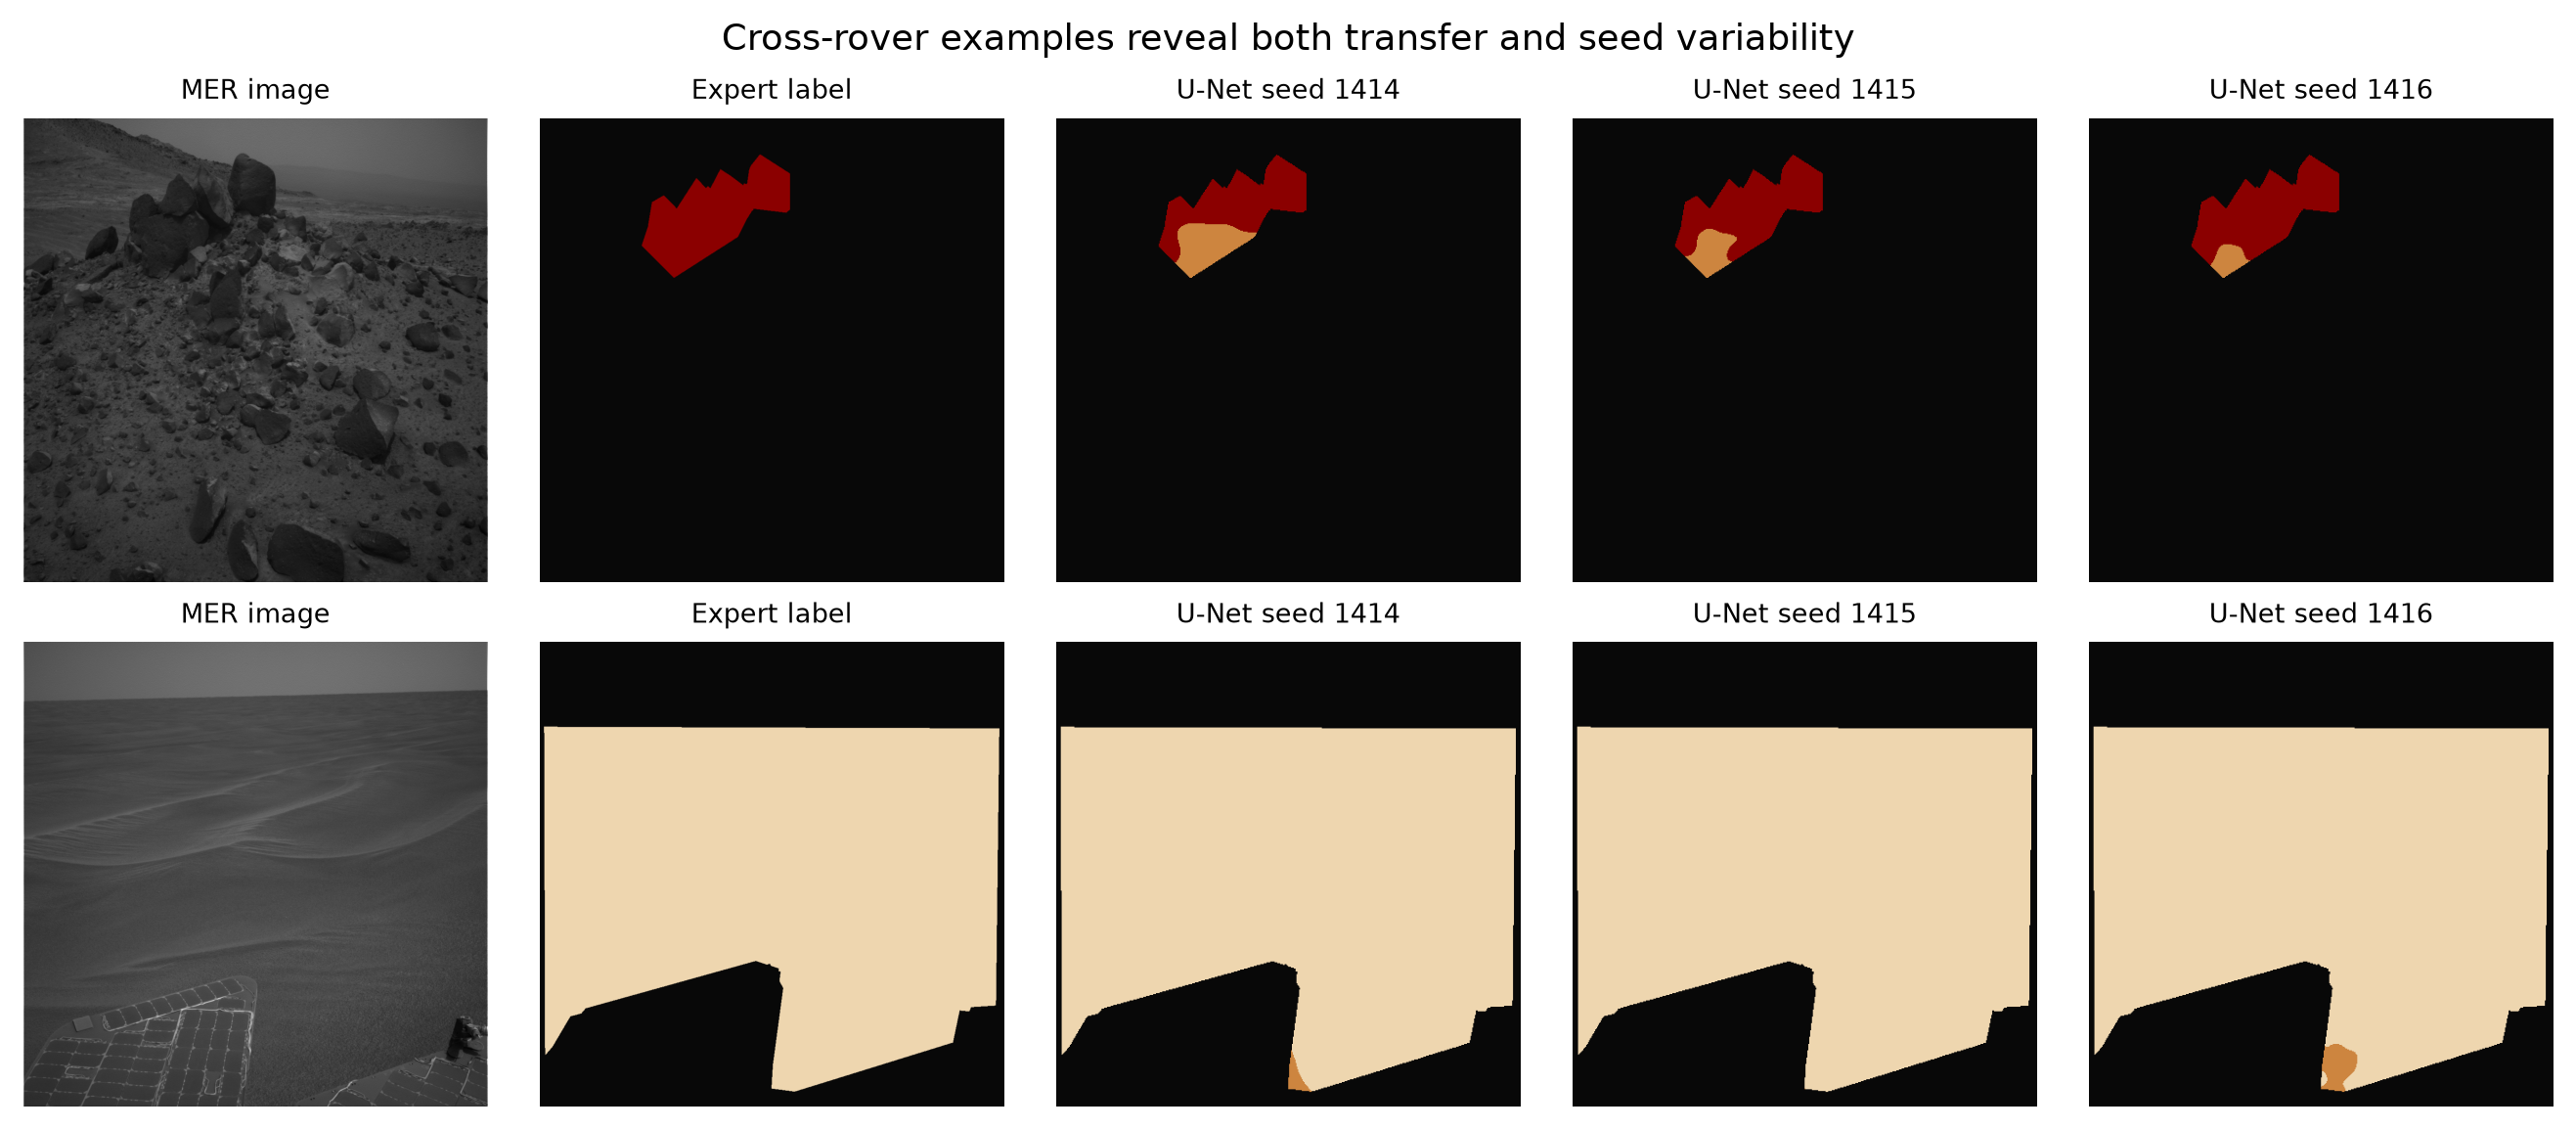
\includegraphics[width=\textwidth]{figures/final/qualitative_mer.png}
  \caption{MER scenes selected for high big-rock (top) and sand (bottom) coverage. The three
  independently trained U-Net checkpoints show where cross-rover predictions are stable and where
  seed variability enters.}
  \label{fig:qual-mer}
\end{figure}

\begin{figure}[h]
  \centering
  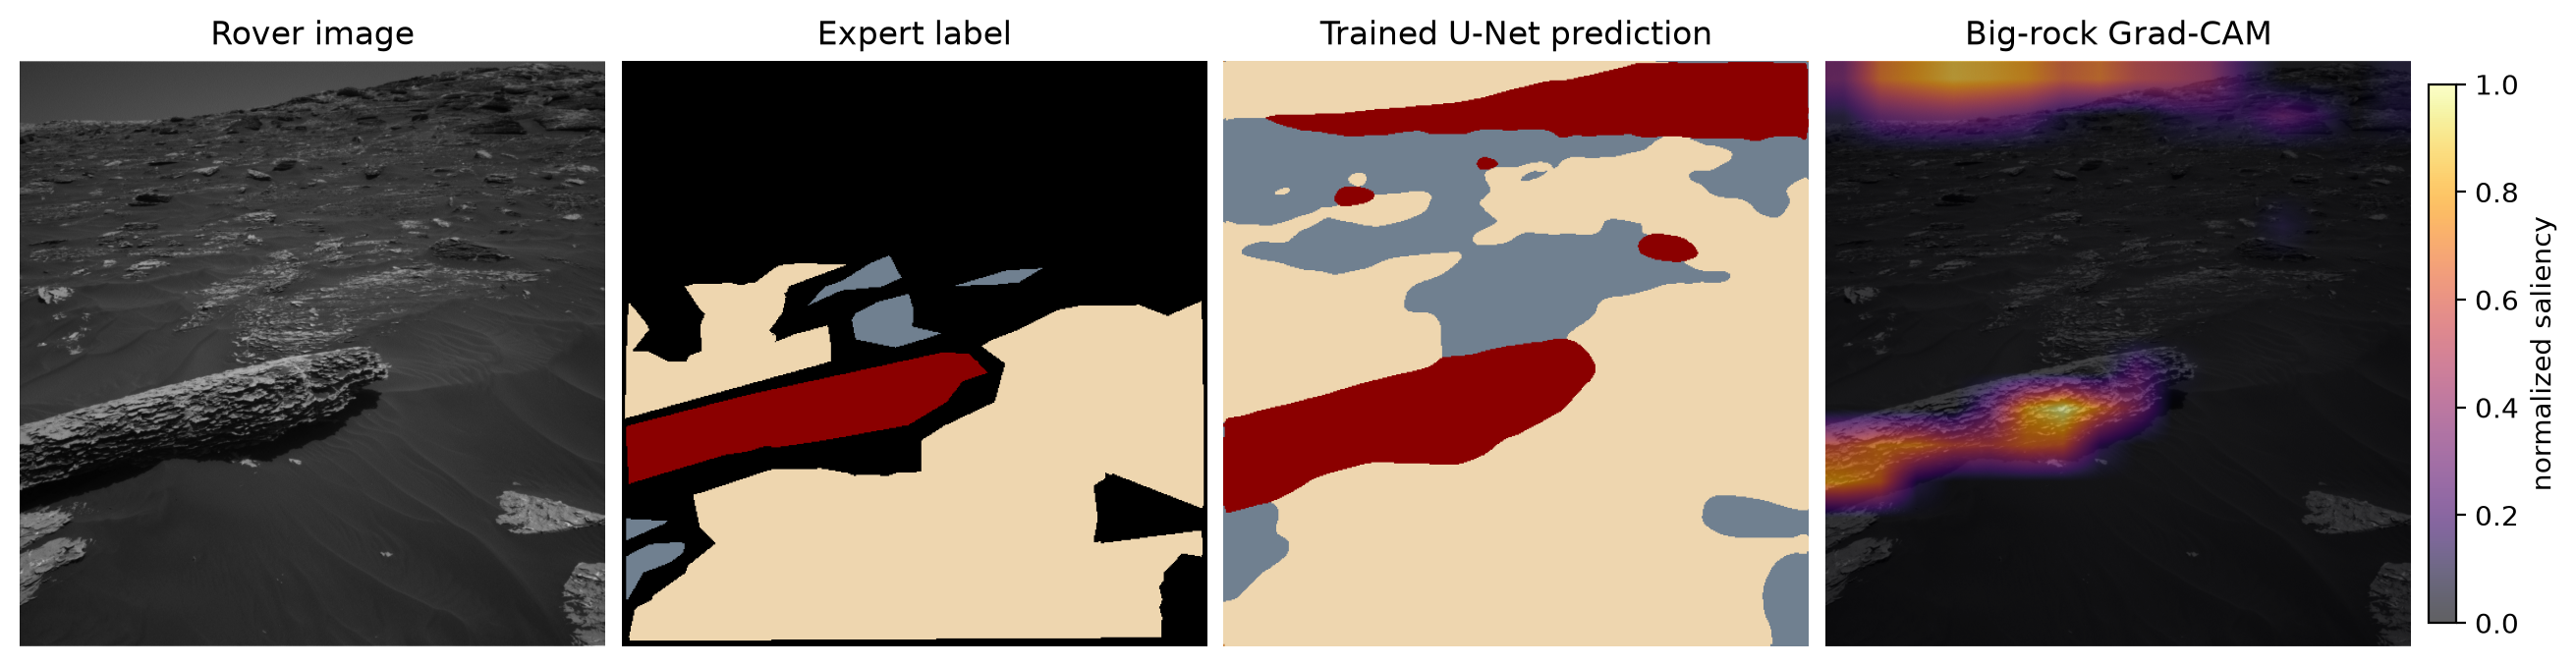
\includegraphics[width=0.86\textwidth]{figures/unet_bigrock_gradcam.png}
  \caption{Gradient-based activation visualization for the U-Net big-rock logit. The map is
  interpretive evidence about spatial sensitivity, not a causal explanation or hypothesis test.}
  \label{fig:gradcam}
\end{figure}

\begin{figure}[h]
  \centering
  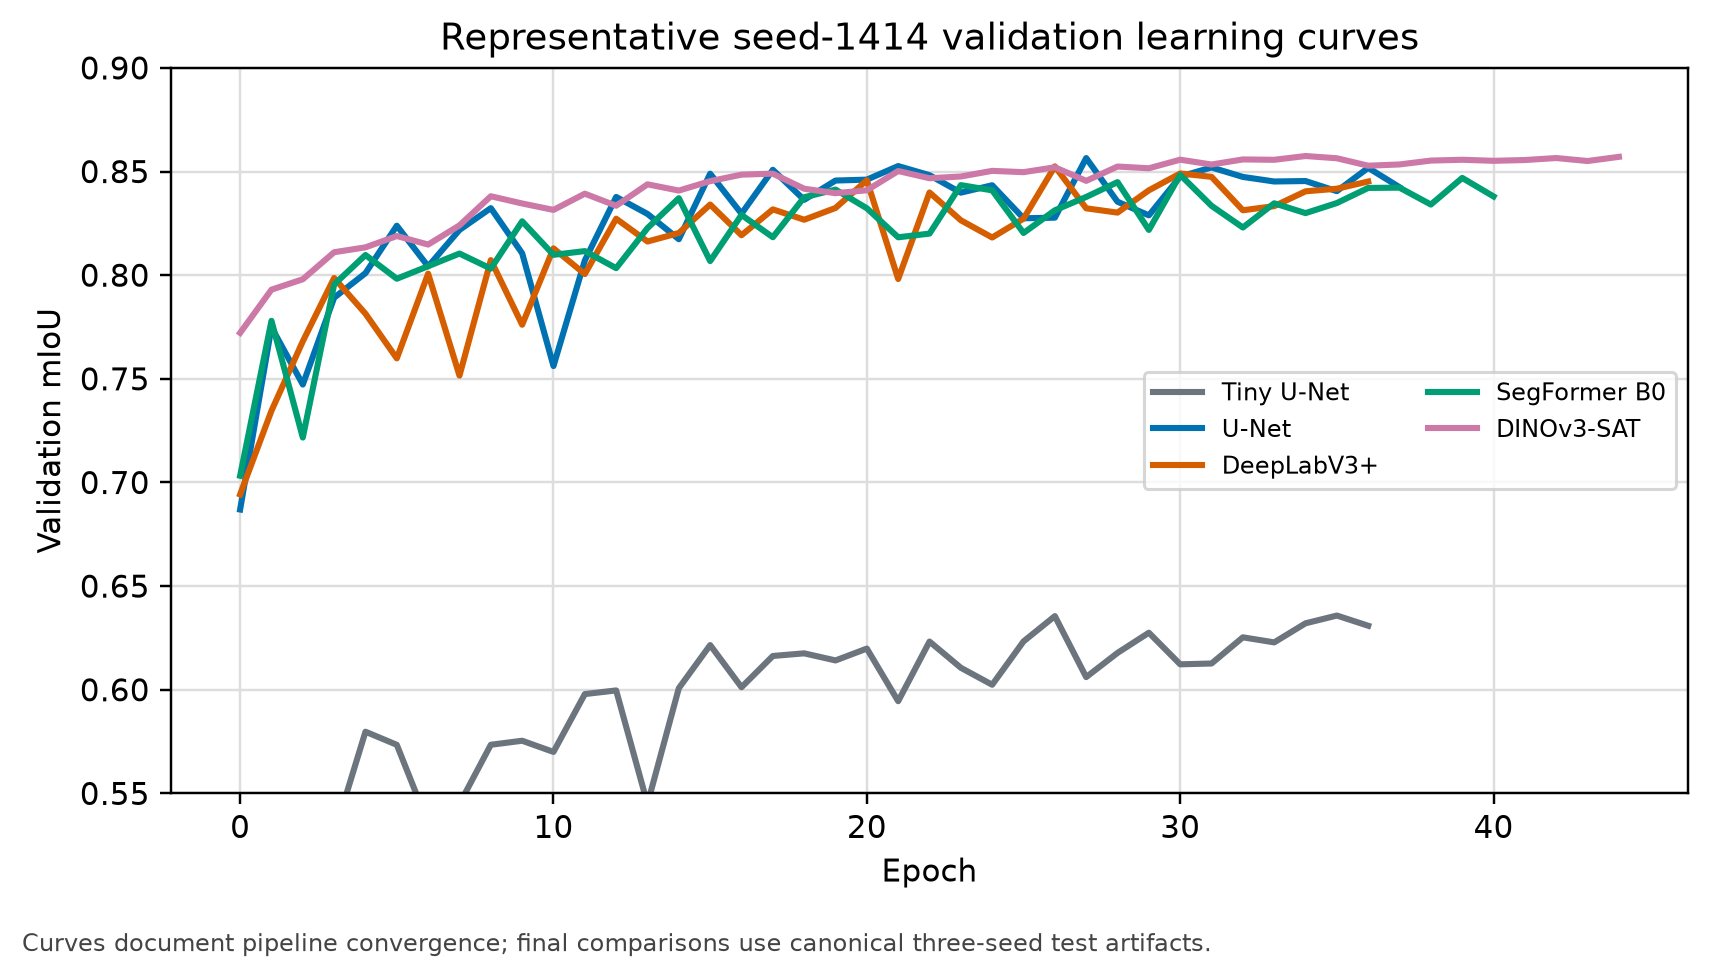
\includegraphics[width=0.86\textwidth]{figures/training_curves.png}
  \caption{Representative seed-1414 validation curves. Final comparisons use the saved best
  checkpoints and all three seeds.}
  \label{fig:curves}
\end{figure}

\section{Exploratory perspective-biased adapter screen}

The Mars Perspective-Biased Adapter (MPBA) screen compared native, content-only, static, raw-$y$,
and learned range-cutoff routing for U-Net and SegFormer-B0 on validation seed 1414. Raw-$y$ gained
0.0071 mean \miou{} over native across backbones and range-cutoff gained 0.0041, but neither met the
joint promotion constraints for big-rock IoU, other-class preservation, latency, and routing use.
No variant was evaluated on the gold test, so the experiment remains exploratory.

\begin{figure}[h]
  \centering
  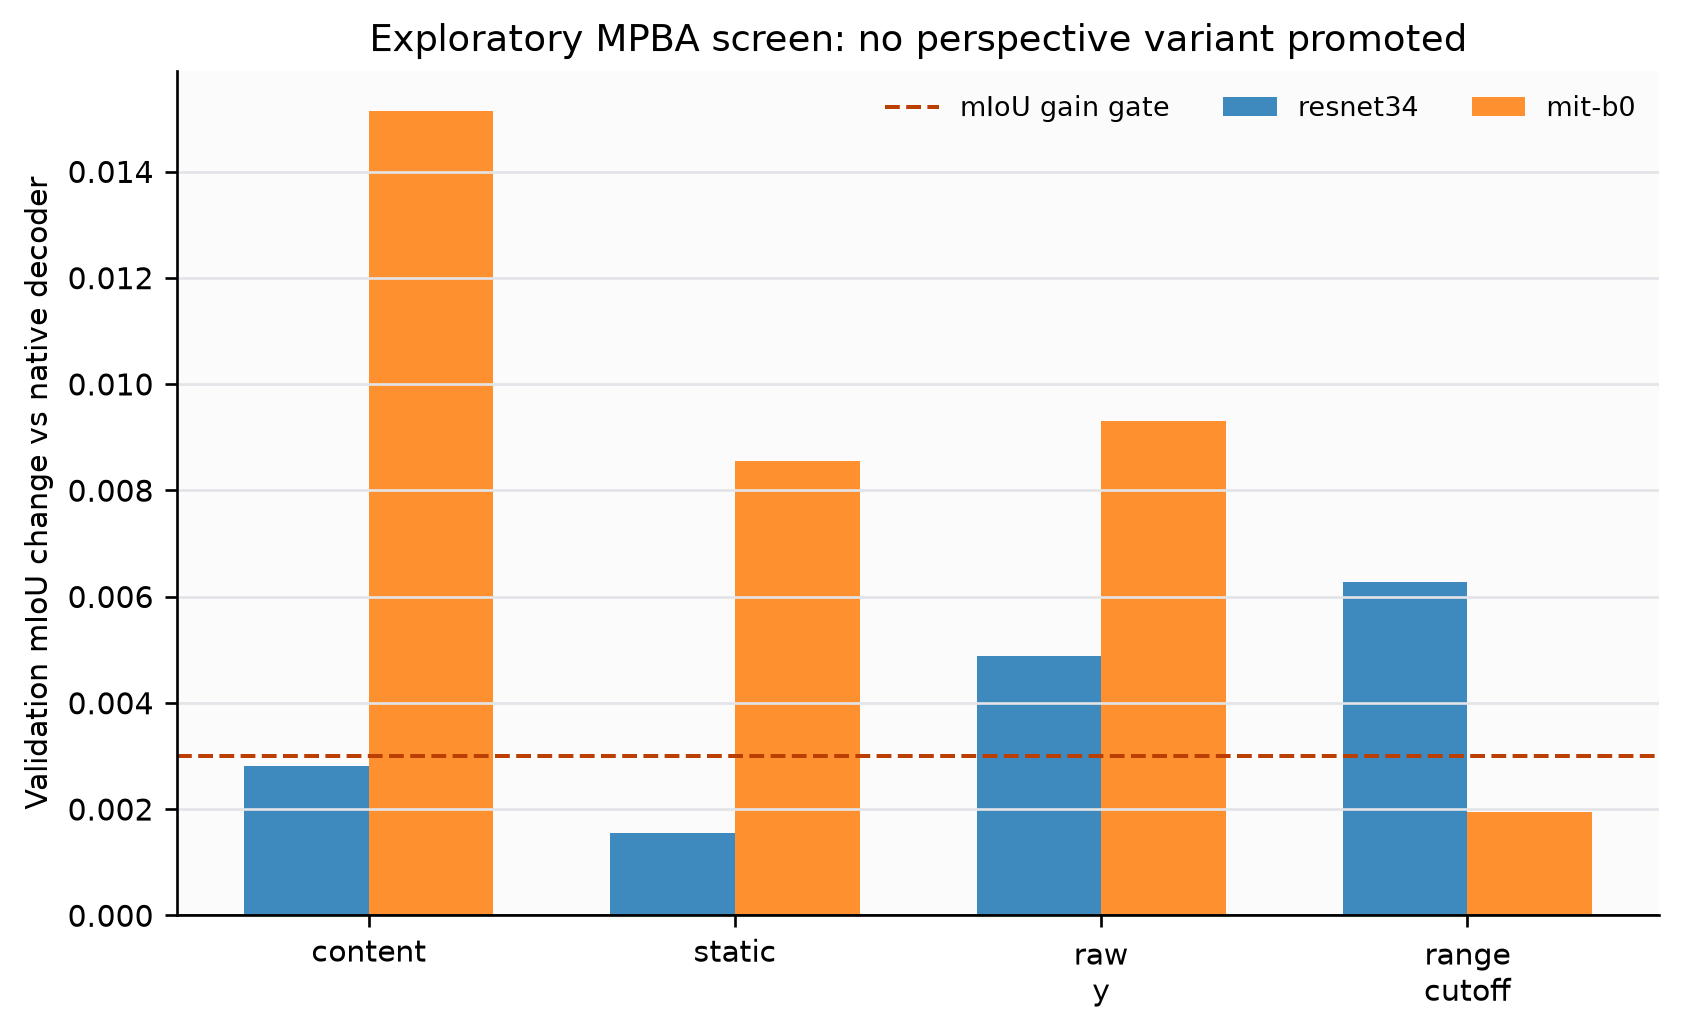
\includegraphics[width=0.78\textwidth]{figures/final/mpba_screen.png}
  \caption{Validation-only MPBA mIoU changes. Crossing the dashed mIoU gate was necessary but not
  sufficient for promotion; no perspective hypothesis passed the complete rule.}
  \label{fig:mpba}
\end{figure}

\section{Protocol amendments and integrity}

The original preregistration and Protocols V2--V4 remain byte-preserved. V4 records the
administrative package rename and permits H4 to reuse only checkpoints with one of three exact
training commits and the exact shared runtime fingerprint. Before any majority prediction, a
fail-closed assertion showed that bedrock, not soil, is the valid training-pixel majority. V5
records the exact counts and changes only the constant predictor from an assumed class to
$\arg\max_c n_c$. The failed attempts produced no manifest, prediction, metric, or result row.
Canonical CSV and Parquet stores contain 328 rows with no duplicate
\code{(run\_id, scope, stratum, metric)} keys.

\section*{NeurIPS Paper Checklist}

\begin{enumerate}

\item \textbf{Claims}
  \item[] Question: Do the main claims made in the abstract and introduction accurately reflect the paper's contributions and scope?
  \item[] Answer: \answerYes{}
  \item[] Justification: The abstract and Sections 1, 5, and 7 report only the sealed H0--H5 decisions and distinguish nonsignificance from equivalence.

\item \textbf{Limitations}
  \item[] Question: Does the paper discuss the limitations of the work performed by the authors?
  \item[] Answer: \answerYes{}
  \item[] Justification: Section 7 discusses dataset, label, seed, domain-shift, compute, oracle-reference, and flight-readiness limitations.

\item \textbf{Theory assumptions and proofs}
  \item[] Question: For each theoretical result, does the paper provide the full set of assumptions and a complete (and correct) proof?
  \item[] Answer: \answerNA{}
  \item[] Justification: The paper is an empirical study and makes no new theoretical claim.

\item \textbf{Experimental result reproducibility}
  \item[] Question: Does the paper fully disclose all the information needed to reproduce the main experimental results of the paper to the extent that it affects the main claims and/or conclusions of the paper?
  \item[] Answer: \answerYes{}
  \item[] Justification: Section 4 gives the data, model, optimization, seed, metric, and inference protocol; sealed configs, manifests, sufficient statistics, and code accompany the paper.

\item \textbf{Open access to data and code}
  \item[] Question: Does the paper provide open access to the data and code, with sufficient instructions to faithfully reproduce the main experimental results, as described in supplemental material?
  \item[] Answer: \answerYes{}
  \item[] Justification: The source repository is public and cites the public Zenodo dataset with acquisition, checksum, layout, and notebook instructions; large raw data and weights are intentionally not duplicated.

\item \textbf{Experimental setting/details}
  \item[] Question: Does the paper specify all the training and test details necessary to understand the results?
  \item[] Answer: \answerYes{}
  \item[] Justification: Sections 3--4 specify splits, image size, augmentations, objective, optimizer, hyperparameters, checkpoint selection, seeds, and test sets.

\item \textbf{Experiment statistical significance}
  \item[] Question: Does the paper report error bars suitably and correctly defined or other appropriate information about the statistical significance of the experiments?
  \item[] Answer: \answerYes{}
  \item[] Justification: Section 4.3 defines the 10,000-replicate seed/image bootstrap, 90\% percentile intervals, plus-one p-values, and Holm families; Section 5 reports intervals and adjusted tests.

\item \textbf{Experiments compute resources}
  \item[] Question: For each experiment, does the paper provide sufficient information on the computer resources needed to reproduce the experiments?
  \item[] Answer: \answerYes{}
  \item[] Justification: Section 4.3 reports V100-SXM2 32 GB hardware, 30 learned runs, 179.1 device-hours, and median run time; manifests retain per-run timestamps and environments.

\item \textbf{Code of ethics}
  \item[] Question: Does the research conducted in the paper conform, in every respect, with the NeurIPS Code of Ethics?
  \item[] Answer: \answerYes{}
  \item[] Justification: The study uses public planetary imagery, reports negative results and amendments, and makes no human-subject or deployment claim.

\item \textbf{Broader impacts}
  \item[] Question: Does the paper discuss both potential positive societal impacts and negative societal impacts of the work performed?
  \item[] Answer: \answerYes{}
  \item[] Justification: Section 7 discusses scientific productivity, rover safety, the harm of confident perception errors, and required deployment safeguards.

\item \textbf{Safeguards}
  \item[] Question: Does the paper describe safeguards that have been put in place for responsible release of data or models that have a high risk for misuse?
  \item[] Answer: \answerNA{}
  \item[] Justification: The project releases no high-risk generative or personal-data model; checkpoints are excluded, and the public planetary dataset is distributed by its original provider.

\item \textbf{Licenses for existing assets}
  \item[] Question: Are the creators or original owners of assets used in the paper properly credited and are the license and terms of use explicitly mentioned and properly respected?
  \item[] Answer: \answerNo{}
  \item[] Justification: All papers, models, NASA/JPL imagery, and the exact Zenodo release are credited, but the bundled merged-0.6 archive metadata does not state an explicit dataset license; Section 7 flags this for downstream verification.

\item \textbf{New assets}
  \item[] Question: Are new assets introduced in the paper well documented and is the documentation provided alongside the assets?
  \item[] Answer: \answerYes{}
  \item[] Justification: The repository documents AresSeg code, configs, notebook, compact result stores, protocol seals, generated figures, and exclusions in its README and development plan.

\item \textbf{Crowdsourcing and research with human subjects}
  \item[] Question: For crowdsourcing experiments and research with human subjects, does the paper include the full text of instructions given to participants and screenshots, if applicable, as well as details about compensation?
  \item[] Answer: \answerNA{}
  \item[] Justification: This study recruited no participants. AI4Mars's prior crowdsourcing is an existing cited public dataset and is not a human-subject experiment conducted here.

\item \textbf{Institutional review board approvals or equivalent}
  \item[] Question: Does the paper describe potential risks incurred by study participants and whether IRB approvals or equivalent were obtained?
  \item[] Answer: \answerNA{}
  \item[] Justification: This study contains no interaction with or data about human subjects.

\item \textbf{Declaration of LLM usage}
  \item[] Question: Does the paper describe the usage of LLMs if it is an important, original, or non-standard component of the core methods in this research?
  \item[] Answer: \answerNA{}
  \item[] Justification: No LLM is part of the dataset, models, experimental method, statistical analysis, or scientific contribution.

\end{enumerate}


\end{document}
